\documentclass[11pt,a4paper]{article}

% ---------------------------------------------------------------------------
% CyberSec-LLM: Fine-Tuning a Compact Domain LLM for Cybersecurity Training
% Compile: pdflatex CyberSecLLM.tex  (run twice for ToC/refs)
% Pure LaTeX + TikZ + pgfplots; no external assets.
% ---------------------------------------------------------------------------

\usepackage[margin=2.2cm]{geometry}
\usepackage[T1]{fontenc}
\usepackage{lmodern}
\usepackage{xcolor}
\usepackage{amsmath,amssymb}
\usepackage{booktabs}
\usepackage{enumitem}
\usepackage{titlesec}
\usepackage{fancyhdr}
\usepackage{listings}
\usepackage{tikz}
\usepackage{pgfplots}
\pgfplotsset{compat=1.18}
\usepackage[hidelinks]{hyperref}
\usetikzlibrary{shapes.geometric, arrows.meta, positioning, fit, backgrounds, calc}

\definecolor{vblack}{HTML}{0A0A0B}
\definecolor{vsoft}{HTML}{17171A}
\definecolor{vgold}{HTML}{D4AF37}
\definecolor{vred}{HTML}{C41E3A}
\definecolor{vreddeep}{HTML}{8B0000}
\definecolor{vslate}{HTML}{2E3440}
\definecolor{vteal}{HTML}{2E6E7E}
\definecolor{codebg}{HTML}{F4F2EC}

\hypersetup{colorlinks=true, linkcolor=vreddeep, urlcolor=vreddeep, citecolor=vreddeep}

\setlength{\headheight}{14pt}
\pagestyle{fancy}
\fancyhf{}
\lhead{\textsc{CyberSec-LLM}}
\rhead{\thepage}
\lfoot{\small Domain-Specialized Compact LLM for Cybersecurity}
\rfoot{\small Technical Report}
\renewcommand{\headrulewidth}{0.5pt}
\renewcommand{\footrulewidth}{0.3pt}

\titleformat{\section}{\Large\bfseries\color{vreddeep}}{\thesection}{0.6em}{}
\titleformat{\subsection}{\large\bfseries\color{vslate}}{\thesubsection}{0.6em}{}

\lstset{
  basicstyle=\ttfamily\small, backgroundcolor=\color{codebg}, breaklines=true,
  frame=single, rulecolor=\color{vslate}, numbers=none, columns=fullflexible,
  keepspaces=true, showstringspaces=false, captionpos=b
}

\tikzset{
  box/.style={rectangle, rounded corners=2pt, draw=vslate, fill=vsoft, text=white,
              minimum height=0.85cm, minimum width=2.5cm, align=center, font=\small},
  gold/.style={draw=vgold, fill=vblack, text=vgold},
  red/.style={draw=vred, fill=vblack, text=vred},
  teal/.style={draw=vteal, fill=vblack, text=white},
  flow/.style={-{Stealth[length=2.2mm]}, draw=vslate, thick},
  goldflow/.style={-{Stealth[length=2.2mm]}, draw=vgold, thick},
  frozen/.style={rectangle, draw=vslate, fill=vslate!30, text=black, minimum height=1.3cm,
                 minimum width=1.5cm, align=center, font=\small},
  train/.style={rectangle, draw=vred, fill=vred!12, text=black, minimum height=0.9cm,
                minimum width=1.2cm, align=center, font=\small}
}

\begin{document}

% ================================================================= TITLE
\begin{titlepage}
\centering
\vspace*{1.5cm}
{\Huge\bfseries\color{vreddeep} CyberSec-LLM\par}
\vspace{0.4cm}
{\Large Fine-Tuning a Compact, Domain-Specialized Language Model\\ for Red/Blue Team Cybersecurity Training\par}
\vspace{0.3cm}
{\large\itshape Technical Report --- Model Architecture, Data, Training, and Evaluation\par}
\vspace{1.6cm}

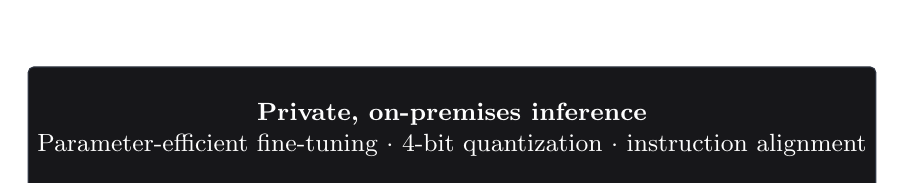
\begin{tikzpicture}
\node[gold, box, minimum width=9cm, minimum height=1.6cm]
  {\textbf{Private, on-premises inference}\\ \small Parameter-efficient fine-tuning $\cdot$ 4-bit quantization $\cdot$ instruction alignment};
\end{tikzpicture}

\vspace{1.4cm}
\begin{tabular}{rl}
\textbf{Objective} & A small ($\leq$3B) instruction-tuned model specialized for the domain\\
\textbf{Method} & QLoRA (4-bit NF4 base + low-rank adapters) supervised fine-tuning\\
\textbf{Base family} & Decoder-only transformer, open-weight, 0.5B--3B parameters\\
\textbf{Deployment} & Quantized artifact served locally behind the platform LLM gateway\\
\textbf{Guarantee} & No training data or inference traffic leaves the institution network\\
\end{tabular}

\vfill
{\small \today\par}
\end{titlepage}

\tableofcontents
\newpage

% ================================================================= 1
\section{Introduction and Motivation}
Large general-purpose language models are unnecessary---and operationally
undesirable---for a supervised cybersecurity training lab. The workload is
narrow and structured: proposing a next reconnaissance/exploitation step,
triaging a SIEM alert into a labelled verdict, mapping activity to a MITRE
ATT\&CK technique, and grading a report against a rubric. These are
\emph{format-constrained, domain-bounded} tasks that a \textbf{compact
model} can perform well once specialized.

We therefore train \textbf{CyberSec-LLM}: a small decoder-only transformer
($\leq 3$B parameters) adapted with parameter-efficient fine-tuning on a
curated cybersecurity instruction corpus. The design targets three properties
simultaneously:

\begin{enumerate}[leftmargin=*]
  \item \textbf{Privacy by construction.} Training and inference execute
        on institution-controlled hardware; no data egresses the network.
  \item \textbf{Task fidelity.} The model reliably emits the strict JSON
        contracts the platform parses, cites ATT\&CK identifiers, and refuses
        out-of-scope requests.
  \item \textbf{Commodity footprint.} A quantized 1.5B--3B model runs at
        interactive latency on modest CPU/GPU hardware.
\end{enumerate}

% ================================================================= 2
\section{Design Goals and Constraints}
\begin{table}[h]
\centering\small
\begin{tabular}{@{}p{4.4cm}p{10.2cm}@{}}
\toprule
\textbf{Requirement} & \textbf{Design consequence}\\
\midrule
On-prem, no egress & Open-weight base; local fine-tune; local inference endpoint only.\\
Small parameter count & Base in the 0.5B--3B range; decoder-only; grouped-query attention where available.\\
Interactive latency & 4-bit weight quantization; short context ($\leq$4k) for copilots; KV-cache reuse.\\
Structured outputs & Supervised fine-tuning on exact JSON schemas; constrained decoding at inference.\\
Reproducibility & Versioned datasets, deterministic seeds, logged prompt/version per call.\\
Safety & Refusal and scope-restriction examples; system-prompt hardening; no offensive payload generation.\\
\bottomrule
\end{tabular}
\caption{Requirements to design mapping.}
\end{table}

% ================================================================= 3
\section{Model Architecture}
CyberSec-LLM uses a standard \textbf{decoder-only transformer} (autoregressive,
causal self-attention). For a token sequence $x_{1:t}$ the model factorizes
the joint probability as
\[
p_\theta(x_{1:T}) \;=\; \prod_{t=1}^{T} p_\theta\!\left(x_t \mid x_{<t}\right),
\]
trained to minimize the token-level cross-entropy (next-token prediction) loss
\[
\mathcal{L}(\theta) \;=\; -\sum_{t} \log p_\theta\!\left(x_t \mid x_{<t}\right).
\]
Each transformer block applies pre-norm multi-head (or grouped-query) attention
followed by a gated feed-forward (SwiGLU) sub-layer with residual connections
and rotary positional embeddings (RoPE):

\begin{figure}[h]
\centering
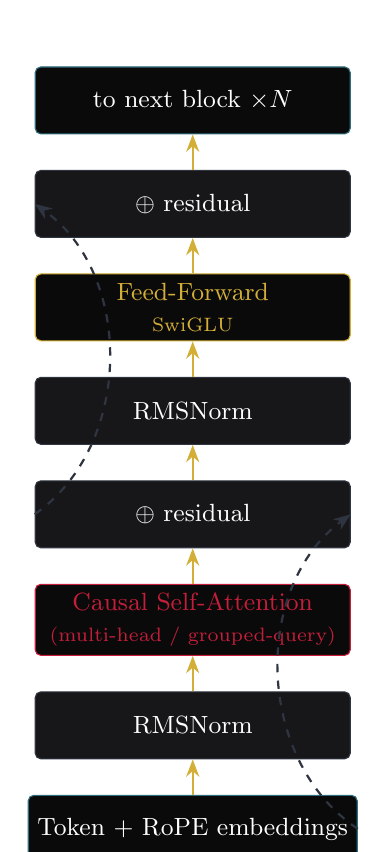
\begin{tikzpicture}[node distance=0.45cm]
  \node[box, teal, minimum width=4cm] (in) {Token + RoPE embeddings};
  \node[box, minimum width=4cm, above=of in] (ln1) {RMSNorm};
  \node[box, red, minimum width=4cm, above=of ln1] (attn) {Causal Self-Attention\\\scriptsize (multi-head / grouped-query)};
  \node[box, minimum width=4cm, above=of attn] (add1) {$\oplus$ residual};
  \node[box, minimum width=4cm, above=of add1] (ln2) {RMSNorm};
  \node[box, gold, minimum width=4cm, above=of ln2] (ff) {Feed-Forward\\\scriptsize SwiGLU};
  \node[box, minimum width=4cm, above=of ff] (add2) {$\oplus$ residual};
  \node[box, teal, minimum width=4cm, above=of add2] (out) {to next block $\times N$};
  \draw[goldflow] (in)--(ln1); \draw[goldflow] (ln1)--(attn);
  \draw[goldflow] (attn)--(add1); \draw[goldflow] (add1)--(ln2);
  \draw[goldflow] (ln2)--(ff); \draw[goldflow] (ff)--(add2); \draw[goldflow] (add2)--(out);
  \draw[flow, dashed] (in.east) to[bend left=55] (add1.east);
  \draw[flow, dashed] (add1.west) to[bend right=55] (add2.west);
\end{tikzpicture}
\caption{One pre-norm decoder block; the stack is repeated $N$ times. Dashed arrows are residual paths.}
\end{figure}

\begin{table}[h]
\centering\small
\begin{tabular}{@{}lccccc@{}}
\toprule
\textbf{Config} & \textbf{Params} & \textbf{Layers} & \textbf{$d_{model}$} & \textbf{Heads} & \textbf{Ctx}\\
\midrule
Tiny  & 0.5B & 24 & 896  & 14 & 32k\\
Small & 1.5B & 28 & 1536 & 12 & 32k\\
Base  & 3.0B & 36 & 2048 & 16 & 128k\\
\bottomrule
\end{tabular}
\caption{Representative compact base configurations (grouped-query attention, RoPE, SwiGLU).}
\end{table}

% ================================================================= 4
\section{Data Engineering}
The corpus is the primary determinant of quality. Every example is stored in a
role-tagged chat format and is designed to reproduce, verbatim, the output
contract of the target platform module.

\begin{lstlisting}[caption={One instruction example (chat JSONL).}]
{"messages":[
  {"role":"system","content":"SOC triage copilot. Reply as JSON."},
  {"role":"user","content":"Suricata: repeated SQLi signatures, one src IP -> web server, 12x/30s."},
  {"role":"assistant","content":"{\"verdict\":\"true_positive\",\"confidence\":0.83,
     \"mitre_technique_id\":\"T1190\",\"next_step\":\"Correlate web logs; block source if confirmed.\"}"}
]}
\end{lstlisting}

\subsection{Corpus composition}
\begin{table}[h]
\centering\small
\begin{tabular}{@{}lcp{7.6cm}@{}}
\toprule
\textbf{Task} & \textbf{Share} & \textbf{What it teaches}\\
\midrule
Pentest next-step (JSON) & 25\% & One safe command + ATT\&CK id, kill-chain ordering.\\
SOC alert triage (JSON) & 25\% & Verdict, confidence, reasoning, response step.\\
MITRE tagging (JSON) & 15\% & Activity/rule $\rightarrow$ single technique id.\\
Report grading (JSON) & 12\% & Rubric-criterion scoring voice.\\
Domain Q\&A (text) & 15\% & Concise explanatory tone.\\
Refusals / scope control & 8\% & Decline out-of-scope or unsafe requests.\\
\bottomrule
\end{tabular}
\caption{Instruction mix (target $\approx$ 1k--3k curated examples).}
\end{table}

\subsection{Data hygiene pipeline}
\begin{enumerate}[leftmargin=*]
  \item \textbf{Schema validation} --- every line parsed; role set and non-empty content enforced.
  \item \textbf{PII / secret scrubbing} --- no real credentials, tokens, or student identifiers; generic placeholders only.
  \item \textbf{Deduplication} --- near-duplicate removal via normalized-text hashing / MinHash to prevent memorization.
  \item \textbf{Decontamination} --- held-out evaluation prompts excluded from the training split.
  \item \textbf{Format conformance} --- JSON-target assistant turns must themselves parse as JSON.
\end{enumerate}

% ================================================================= 5
\section{Fine-Tuning Methodology: QLoRA}
We use \textbf{QLoRA}---low-rank adaptation on top of a 4-bit-quantized frozen
base---to specialize the model at a fraction of full fine-tuning cost.

\subsection{Low-rank adaptation (LoRA)}
For a pretrained weight $W_0 \in \mathbb{R}^{d\times k}$, LoRA constrains the
update to a low-rank product and freezes $W_0$:
\[
W \;=\; W_0 \;+\; \Delta W, \qquad \Delta W = \frac{\alpha}{r}\, B A,\quad
B \in \mathbb{R}^{d\times r},\; A \in \mathbb{R}^{r\times k},\; r \ll \min(d,k).
\]
The forward pass becomes $h = W_0 x + \frac{\alpha}{r} B(Ax)$. Only $A,B$ are
trained, reducing trainable parameters from $dk$ to $r(d{+}k)$. With
$r{=}16$ this is typically \textbf{$<1\%$} of model parameters.

\subsection{4-bit base (NF4) and paged optimization}
The frozen base is stored in 4-bit \emph{NormalFloat} (NF4), dequantized
on-the-fly during the forward/backward pass; adapter weights and optimizer
states remain in higher precision. Gradient checkpointing and 8-bit optimizer
states further cut memory, letting a 3B model fine-tune within a single
$\sim$16\,GB accelerator.

\begin{figure}[h]
\centering
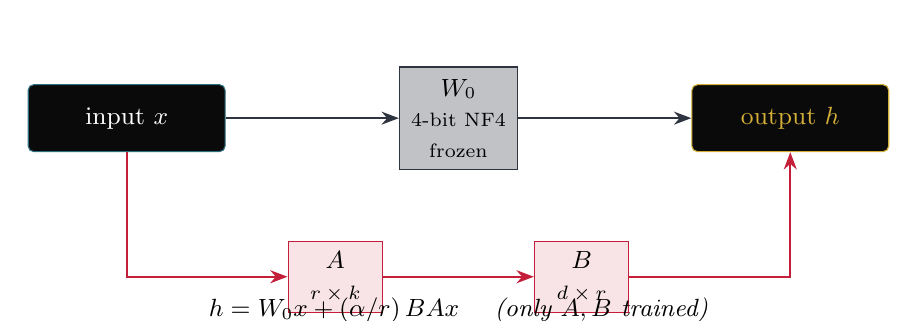
\begin{tikzpicture}[node distance=0.7cm]
  \node[frozen] (w0) {$W_0$\\\scriptsize 4-bit NF4\\\scriptsize frozen};
  \node[train, below left=0.9cm and 0.2cm of w0] (a) {$A$\\\scriptsize $r\times k$};
  \node[train, below right=0.9cm and 0.2cm of w0] (b) {$B$\\\scriptsize $d\times r$};
  \node[box, teal, left=2.2cm of w0] (x) {input $x$};
  \node[box, gold, right=2.2cm of w0] (h) {output $h$};
  \draw[flow] (x) -- (w0);
  \draw[flow] (w0) -- (h);
  \draw[flow, vred] (x.south) |- (a.west);
  \draw[flow, vred] (a) -- (b);
  \draw[flow, vred] (b.east) -| (h.south);
  \node[below=1.5cm of w0, font=\small\itshape] {$h = W_0 x + (\alpha/r)\,B A x$ \quad (only $A,B$ trained)};
\end{tikzpicture}
\caption{QLoRA: a frozen 4-bit base with trainable low-rank adapters injected into the attention/MLP projections.}
\end{figure}

\subsection{Hyperparameters}
\begin{table}[h]
\centering\small
\begin{tabular}{@{}ll l l@{}}
\toprule
\textbf{Parameter} & \textbf{Value} & \textbf{Parameter} & \textbf{Value}\\
\midrule
LoRA rank $r$ & 16 & Optimizer & AdamW (8-bit)\\
LoRA $\alpha$ & 16 & Learning rate & $2\times10^{-4}$\\
LoRA dropout & 0.0 & LR schedule & linear w/ warmup\\
Target modules & \texttt{q,k,v,o,gate,up,down} & Epochs & 2--3\\
Base precision & 4-bit NF4 & Batch (eff.) & 8 (2$\times$4 accum.)\\
Max seq length & 4096 & Weight decay & 0.01\\
Grad checkpoint & on & Seed & fixed\\
\bottomrule
\end{tabular}
\caption{QLoRA supervised fine-tuning configuration.}
\end{table}

% ================================================================= 6
\section{Training Pipeline}
\begin{figure}[h]
\centering
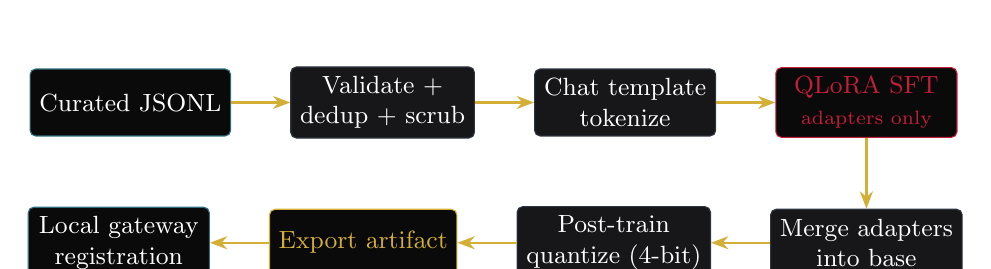
\begin{tikzpicture}[node distance=0.55cm and 0.75cm]
  \node[box, teal, minimum width=2.3cm] (raw) {Curated JSONL};
  \node[box, right=of raw, minimum width=2.3cm] (val) {Validate +\\dedup + scrub};
  \node[box, right=of val, minimum width=2.3cm] (tmpl) {Chat template\\tokenize};
  \node[box, red, right=of tmpl, minimum width=2.3cm] (sft) {QLoRA SFT\\\scriptsize adapters only};
  \node[box, below=0.9cm of sft, minimum width=2.3cm] (merge) {Merge adapters\\into base};
  \node[box, left=of merge, minimum width=2.3cm] (quant) {Post-train\\quantize (4-bit)};
  \node[box, gold, left=of quant, minimum width=2.3cm] (pkg) {Export artifact};
  \node[box, teal, left=of pkg, minimum width=2.3cm] (serve) {Local gateway\\registration};
  \draw[goldflow] (raw)--(val); \draw[goldflow] (val)--(tmpl); \draw[goldflow] (tmpl)--(sft);
  \draw[goldflow] (sft)--(merge); \draw[goldflow] (merge)--(quant);
  \draw[goldflow] (quant)--(pkg); \draw[goldflow] (pkg)--(serve);
\end{tikzpicture}
\caption{End-to-end pipeline: data preparation, adapter training, merge, quantization, and local registration.}
\end{figure}

% ================================================================= 7
\section{Alignment and Safety}
Because the model advises on offensive and defensive security, alignment is a
first-class training objective, not an afterthought:
\begin{itemize}[leftmargin=*]
  \item \textbf{Scope restriction.} Explicit examples teach the model to refuse
        targets outside the isolated lab range and to never emit destructive or
        novel exploit payloads---only orchestration of documented tooling.
  \item \textbf{Human-in-the-loop framing.} The pentest task never ``executes'';
        it proposes a single action for human approval, reinforced in every
        training example.
  \item \textbf{Contract adherence.} JSON-only targets reduce prompt-injection
        surface and make outputs machine-verifiable.
  \item \textbf{Adversarial evaluation.} The model is probed post-training with
        prompt-injection and jailbreak suites; failures feed the next data
        iteration (a closed hardening loop).
\end{itemize}

% ================================================================= 8
\section{Quantization and Footprint}
Post-training weight quantization to 4-bit reduces the served artifact roughly
$4\times$ versus fp16 while preserving task accuracy for these constrained
outputs. Approximate resident weight memory $M \approx N \cdot b / 8$ bytes for
$N$ parameters at $b$ bits:

\begin{table}[h]
\centering\small
\begin{tabular}{@{}lccc@{}}
\toprule
\textbf{Model} & \textbf{fp16 ($\approx$)} & \textbf{4-bit ($\approx$)} & \textbf{QLoRA train VRAM}\\
\midrule
0.5B & 1.0 GB & 0.30 GB & $\sim$4 GB\\
1.5B & 3.0 GB & 0.90 GB & $\sim$7 GB\\
3.0B & 6.0 GB & 1.7 GB  & $\sim$12 GB\\
\bottomrule
\end{tabular}
\caption{Approximate weight footprint and single-accelerator training budget.}
\end{table}

% ================================================================= 9
\section{Evaluation Protocol}
Evaluation is task-specific and automated where possible, on a decontaminated
held-out split. Metrics:
\begin{itemize}[leftmargin=*]
  \item \textbf{JSON validity rate} --- fraction of copilot outputs that parse against the module schema.
  \item \textbf{MITRE tagging accuracy} --- exact-match technique id vs.\ gold labels.
  \item \textbf{SOC verdict F1} --- macro-F1 over \{true positive, false positive, benign\} vs.\ faculty ground truth.
  \item \textbf{Refusal correctness} --- correct decline on out-of-scope/unsafe prompts.
  \item \textbf{Perplexity} --- held-out next-token loss for regression tracking.
\end{itemize}

\begin{figure}[h]
\centering
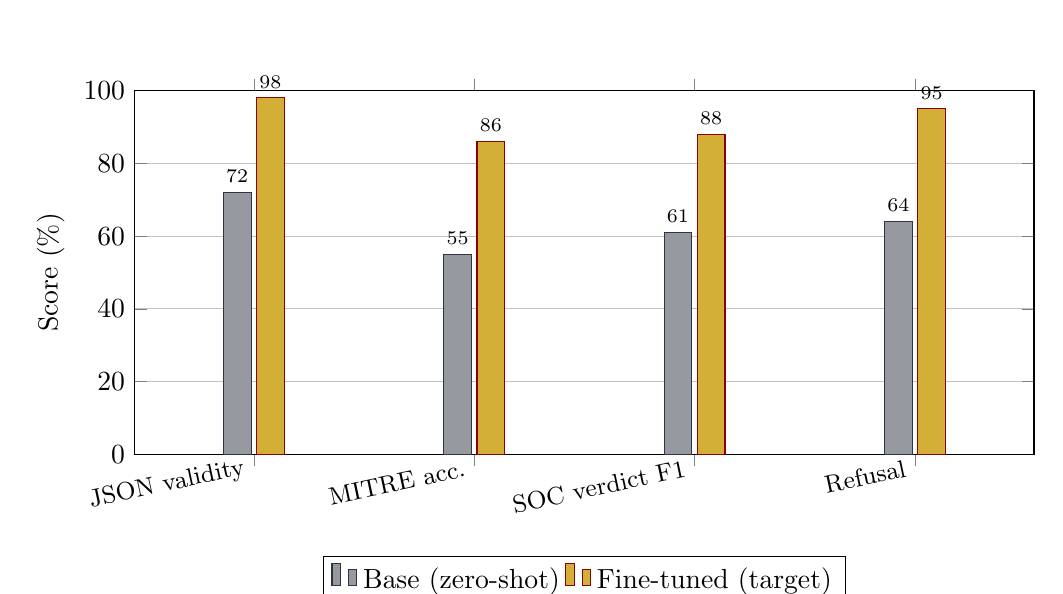
\begin{tikzpicture}
\begin{axis}[
  ybar, bar width=10pt, width=13cm, height=6.2cm,
  ymin=0, ymax=100, ylabel={Score (\%)},
  symbolic x coords={JSON validity, MITRE acc., SOC verdict F1, Refusal},
  xtick=data, x tick label style={font=\small, rotate=12, anchor=east},
  legend style={at={(0.5,-0.28)}, anchor=north, legend columns=-1},
  enlarge x limits=0.18, ymajorgrids, grid style={vslate!30},
  nodes near coords, every node near coord/.append style={font=\scriptsize},
]
\addplot[fill=vslate!50, draw=vslate] coordinates
  {(JSON validity,72) (MITRE acc.,55) (SOC verdict F1,61) (Refusal,64)};
\addplot[fill=vgold, draw=vreddeep] coordinates
  {(JSON validity,98) (MITRE acc.,86) (SOC verdict F1,88) (Refusal,95)};
\legend{Base (zero-shot), Fine-tuned (target)}
\end{axis}
\end{tikzpicture}
\caption{Acceptance targets: parameter-efficient fine-tuning chiefly improves format conformance, tagging, and refusal reliability. Values are target thresholds for release sign-off, not a claim of a specific trained checkpoint.}
\end{figure}

% ================================================================= 10
\section{Inference and Integration}
The released artifact is served on institution hardware behind the platform's
LLM gateway over an HTTP interface; no third-party service is contacted. The
gateway performs module-aware routing, injects the versioned system prompt,
enforces a per-session token budget, and logs the full prompt/completion pair
with the prompt version for reproducibility. Inference-time reliability is
further improved with constrained/JSON-guided decoding and a low sampling
temperature for the structured tasks.

% ================================================================= 11
\section{Compute Budget}
\begin{itemize}[leftmargin=*]
  \item \textbf{Training} (one-time, per model version): a single mid-range
        accelerator; on the order of 1--3 GPU-hours for 1.5B--3B with QLoRA on
        a few thousand examples.
  \item \textbf{Inference} (continuous): a 4-bit 1.5B--3B model runs at
        interactive latency on a modest GPU, and acceptably on multi-core CPU
        for the short-context copilot tasks.
\end{itemize}

% ================================================================= 12
\section{Reproducibility and Governance}
Every model version is tied to (i) an immutable dataset snapshot, (ii) the exact
hyperparameter set and random seed, and (iii) a registry entry recording the
served model name and the system-prompt version. Because the platform logs the
prompt version and model on every call, any graded artifact can be reproduced
and audited---an explicit requirement for accreditation evidence.

% ================================================================= 13
\section{Limitations and Future Work}
\begin{itemize}[leftmargin=*]
  \item Fine-tuning primarily shapes \emph{style, format, and domain grounding};
        factual recall is better served by retrieval augmentation over a
        curated knowledge base.
  \item Small models have finite reasoning depth; complex multi-step
        exploitation reasoning should remain human-supervised.
  \item Planned: preference optimization (DPO) on faculty-rated outputs;
        retrieval-augmented generation over ATT\&CK and course materials;
        distillation from a larger local teacher; per-technique attainment
        calibration.
\end{itemize}

\vspace{0.8cm}
\begin{center}\small\itshape End of technical report --- CyberSec-LLM.\end{center}

\end{document}
